%!TEX root = RBM.tex

\subsection{Estimating Results}

We estimate the results of the three algorithms using 4 models with 10, 20, 100, 500 hidden units respectively, all 4 models have 784 visible units. The models are trained by the MNIST handwritten digit dataset\cite{lecun1998mnist}.

Note that we only calculate the real value of the partition function in the model with 10 hidden units ($logZ(\theta)=226.11$), due to my poor laptop has broken down several times when calculating the model with 20 hidden units and maltab doesn't even allow to calculate the other two models because they require unimaginable quantity of memories.

\para{AIS}
\begin{table}[t]
\centering
{\small
\begin{tabular}{c|ccc}
    \hline
    \textbf{Hid Units} & \textbf{Mean $logZ(\theta)$} & \textbf{+/-3 sd} & \textbf{Real Value} \\ 
    \hline
	   10  & 226.05 & 0.1762 & 226.11 \\
	   20  & 221.11 & 0.2329 & N/A 	  \\
	   100 & 348.45 & 0.2460 & N/A 	  \\
	   500 & 463.25 & 0.3790 & N/A 	  \\ \hline
\end{tabular}
}
\vspace{-0.1in}
\caption{AIS result (with $\mathbf b$ init) with $+/-3$ standard deviations}
\label{tab:aisresult}
% \vspace{-0.05in}
\end{table}
By setting $\mathbf \beta$ uniformly sampling from 0 to 1 for 10,000 points, we run 100 times of AIS, and get a result with $+/-3$ standard deviations (Table~\ref{tab:aisresult}). In a model with 10 hidden units. We see AIS with init almost obtain the real value (226.11) without error.

\begin{figure}[t]
	\centering
	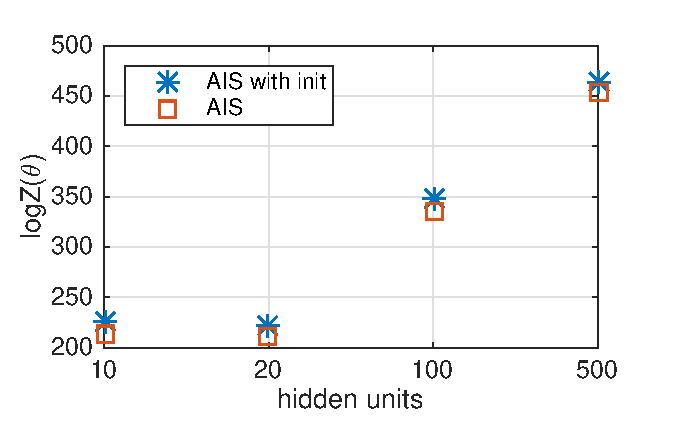
\includegraphics[width=0.48\textwidth]{figure/AIS_results/ais_result.eps}
% \vspace{-0.1in}
	\caption{Comparison of AIS method, with or without an initialization of $\mathbf b$}
\label{fig:aisinit} % FIG1
\end{figure}
From Figure~\ref{fig:aisinit}, we can see that the estimation results will differ a lot if we use an initialization method to initialize the visible bias $\mathbf b$, as mentioned in the previous subsection. And from the validation of the 10 hidden units case, we can infer that with a initialization of $\mathbf b$ would largely improve the result.




\para{RTS}
When doing the practice of RTS, as mentioned in the last subsection, we directly use the initializing method mentioned above by selecting $\beta_{k}$ with a uniform distribution in every loop. Also, we use the same initialization method as in AIS to initialize $\mathbf b$ in model A. 

We make 50 transitions from $x_{k}$ to $x_{k+1}$ in every loop, we take 100 loops (i.e.$N=100$) every time, and we conduct the whole procedure for 100 times (i.e.we update $\mathbf Z$ for 100 times). Also, we select 100 point of $\mathbf \beta$ uniformly sampled from 0 to 1. 

By conducting the whole above procedure for 20 times, we can obtain a result which is as good as AIS (Table~\ref{tab:allresult}). However, the efficiency of RTS show weaker performance than that of AIS (Table~\ref{tab:efficiencyresult}).

\para{TAP}
\begin{figure}[t]
\begin{minipage}[t]{1\linewidth}
	\centering
  	\subfigure{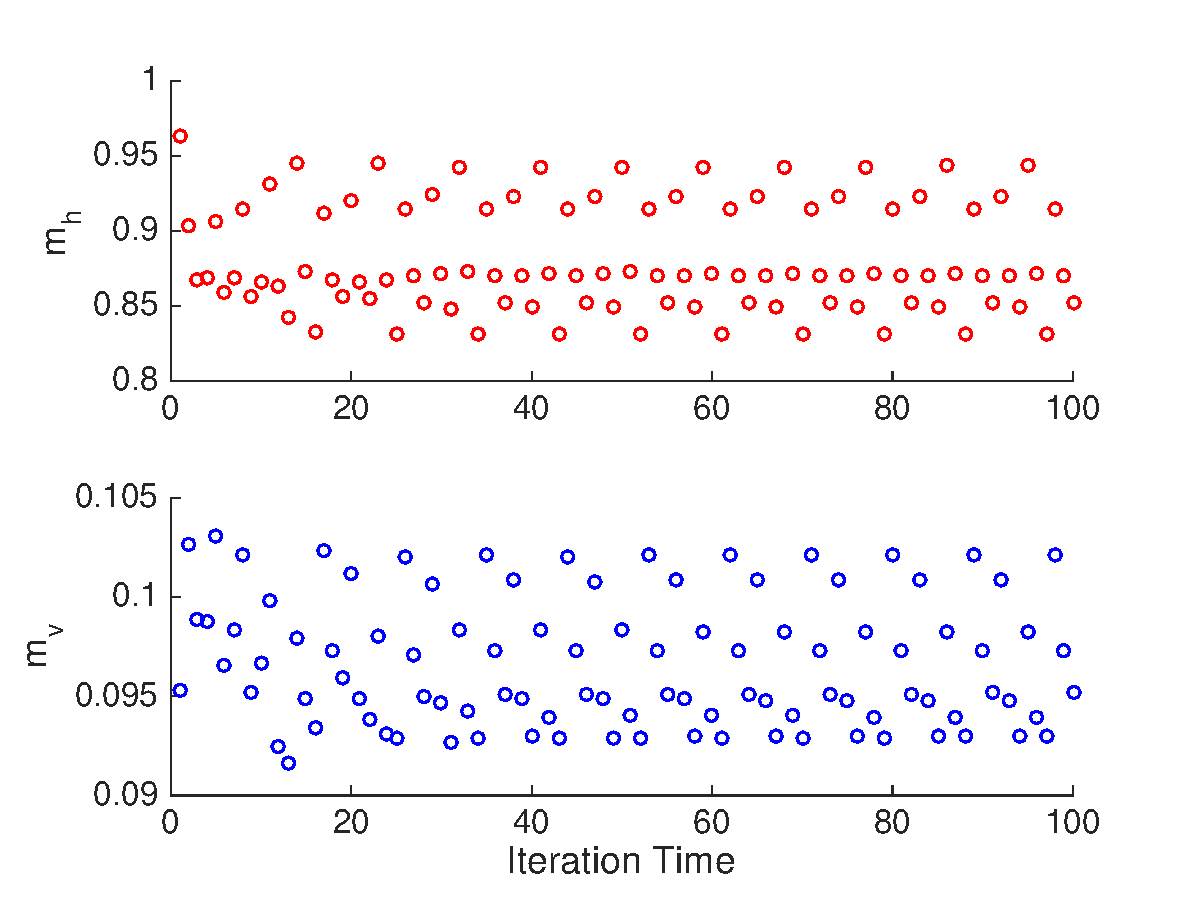
\includegraphics[width=0.48\textwidth]{figure/TAP_results/mvmh_10.eps}}
	\subfigure{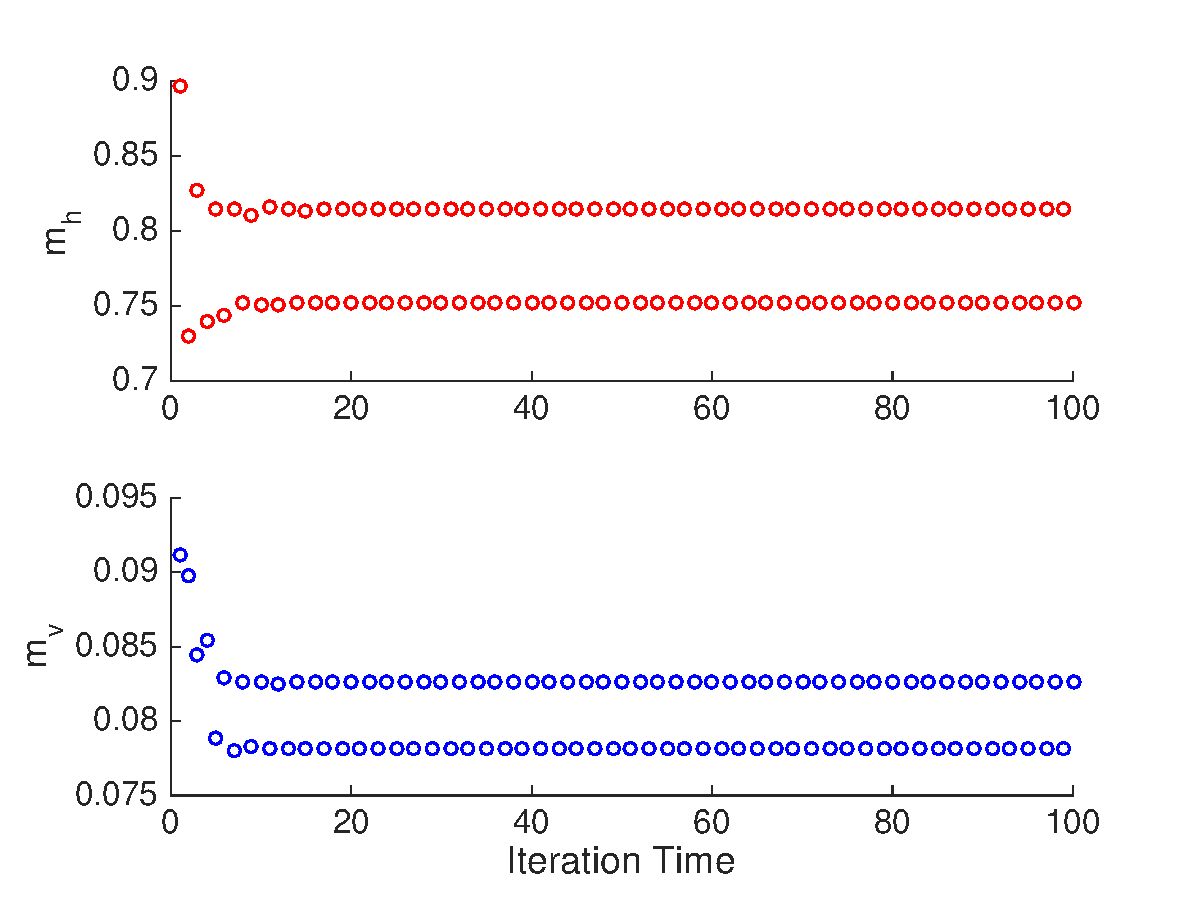
\includegraphics[width=0.48\textwidth]{figure/TAP_results/mvmh_20.eps}}
	\subfigure{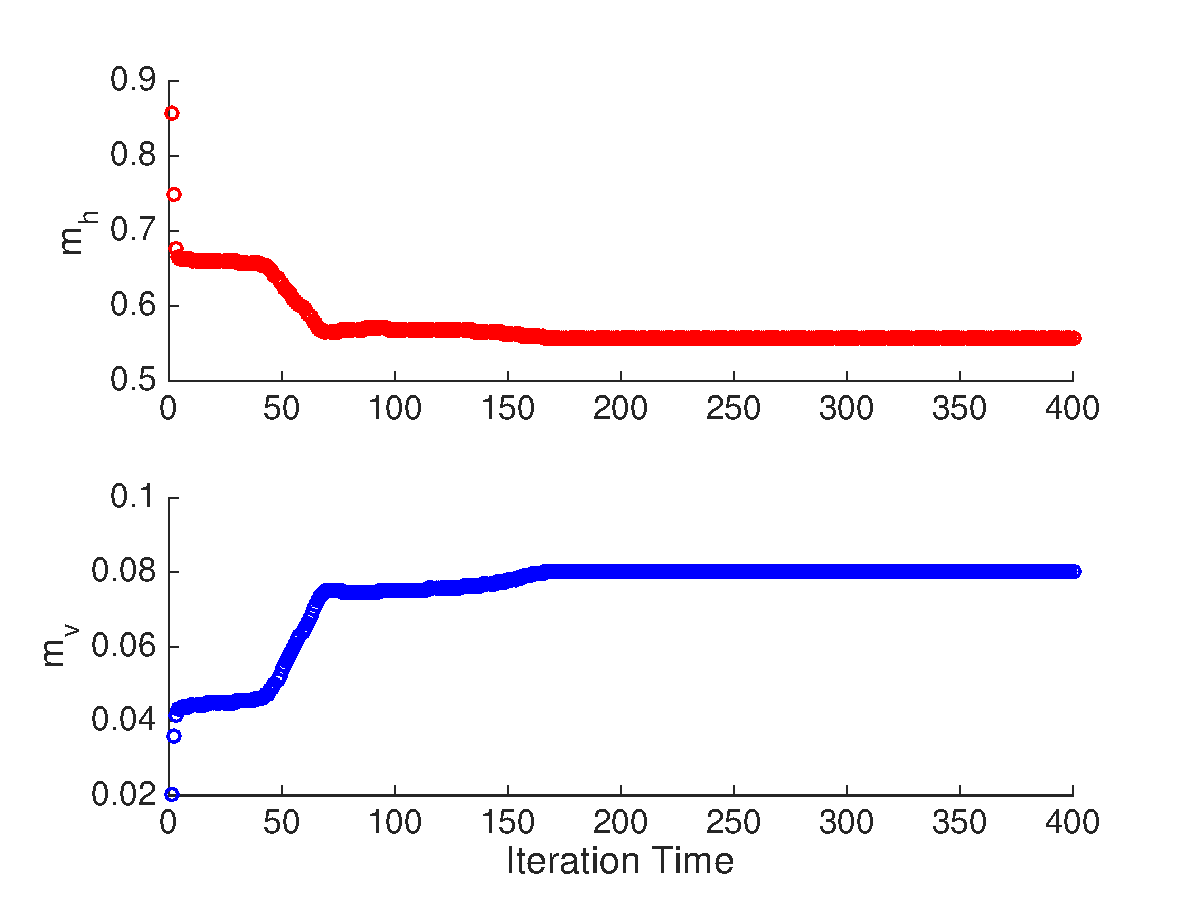
\includegraphics[width=0.48\textwidth]{figure/TAP_results/mvmh_100.eps}}
	\subfigure{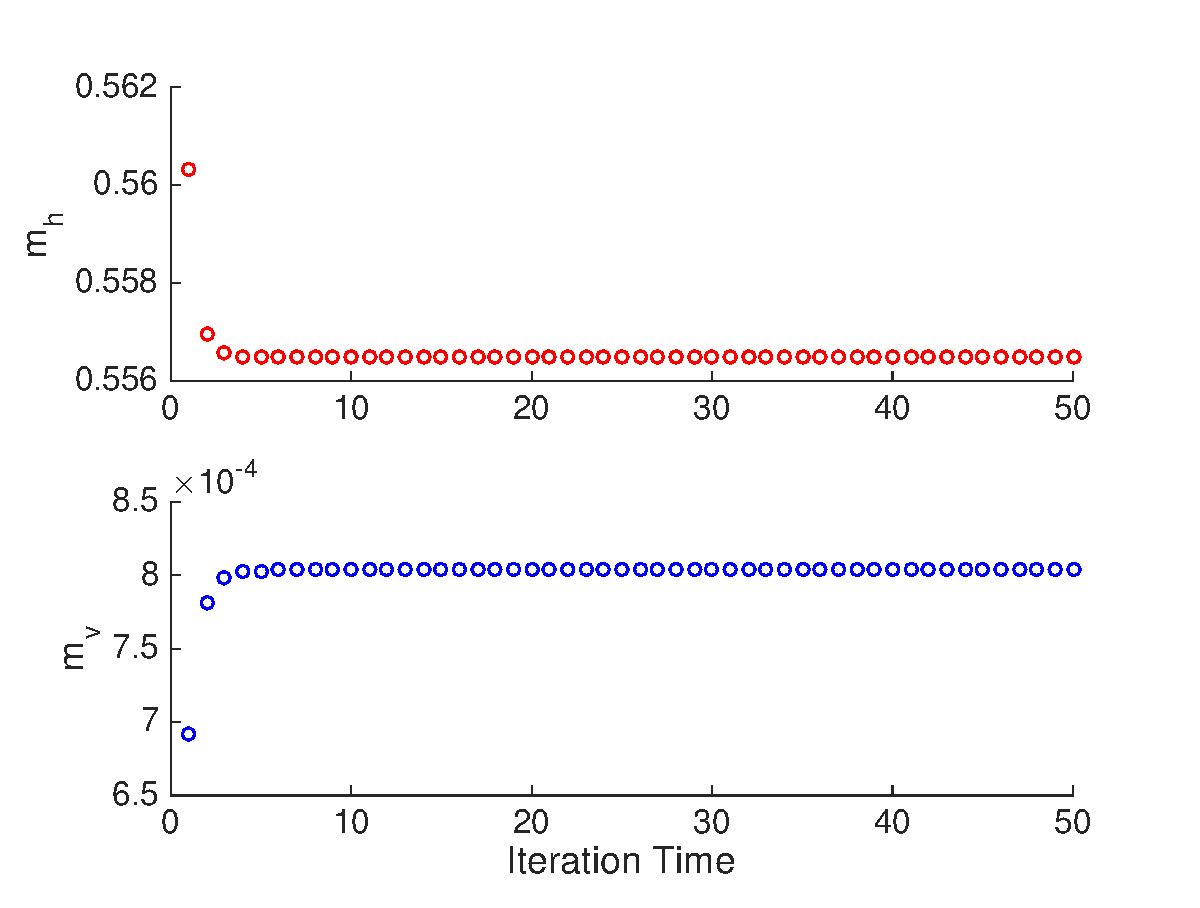
\includegraphics[width=0.48\textwidth]{figure/TAP_results/mvmh_500.eps}}
% \vspace{-0.1in}
\caption{$m_{h}$, $m_{v}$ convergence condition using TAP method. From left to right, up to down, the figure indicates an RBM model with 10, 20, 100, 500 hidden units. The convergence time is approximately 40, 20, 175, 5. By such few iteration time, all results can be obtained in less than 1 second.}
\label{fig:TAPmhmviter} % FIG1
\end{minipage}
\vspace{-0.05in}
\end{figure}
When running a TAP, we see we can get converged $m_{v}$ \& $m_{h}$ in very few iteration time (Figure~\ref{fig:TAPmhmviter}, convergence time is approximately 40, 20, 175, 5 for the model with 10, 20, 100, 500 hidden units respectively). Given this observation, the computing time of TAP is negligeable (we obtain all results in less than a second). And also, its meaningless to discuss standard deviation here.

However, we do notice that the converged results are sometimes not consistent but periodic. (eg. Figure~\ref{fig:TAPmhmviter}, when there are 10, 20 hidden units), this is not a good news because even if we have more resources to compute the iterations, we would not have a better result.

\begin{table}[t]
\centering
{\small
\begin{tabular}{c|ccccc}
    \hline
    \textbf{Hid Units} & \textbf{TAP} & \textbf{AIS} & \textbf{RTS} & \textbf{Real Value} \\ 
    \hline
	   10  & 212.32 & 226.05 & 226.2707 & 226.11 	  \\
	   20  & 214.85 & 221.11 & 218.8993 & N/A 	  \\
	   100 & 342.02 & 348.45 & 347.3684 & N/A 	  \\
	   500 & 450.31 & 463.25 & 459.7372 & N/A 	  \\ \hline
\end{tabular}
}
\vspace{-0.1in}
\caption{$Z(\theta)$ estimation result of TAP, AIS, RTS (AIS \& RTS with $\mathbf b$ init)}
\label{tab:allresult}
% \vspace{-0.05in}
\end{table}
\begin{table}[t]
\centering
{\small
\begin{tabular}{c|ccccc}
    \hline
    \textbf{Hid Units} & \textbf{TAP} & \textbf{AIS} & \textbf{RTS} \\ 
    \hline
	   10  & < 1 & 77.38 & 68.28  \\
	   20  & < 1 & 63.03 & 87.42  \\
	   100 & < 1 & 92.87 & 164.34 \\
	   500 & < 1 & 154.63 & 603.59 \\ \hline
\end{tabular}
}
\vspace{-0.1in}
\caption{Efficiency of TAP, AIS, RTS (Unit: seconds), with a Intel Core i5 CPU Turbo Boost to 2.7GHz}
\label{tab:efficiencyresult}
% \vspace{-0.05in}
\end{table}

And disappointingly, compared to the result of other algorithms (Table~\ref{tab:allresult}), TAP usually have a lower estimation value, which is not preferable.







